\documentclass[fleqn,10pt]{olplainarticle}
\usepackage{graphicx}
\usepackage{subcaption}
\usepackage{hyperref}
\usepackage{cleveref}
\usepackage{placeins}
\crefname{subsection}{subsection}{subsections}
\Crefname{subsection}{Subsection}{Subsections}


\title{Boundary effects in spatial graphs}
\author[1]{First Author}
\author[2]{Second Author}
\affil[1]{Address of first author}
\affil[2]{Address of second author}

\keywords{Keyword1, Keyword2, Keyword3}

\begin{abstract}
Package: bosperrus: \textbf{bo}rder effects in \textbf{sp}atial graphs: \textbf{err}or modelling and \textbf{u}ntangling \textbf{s}trategies.
\end{abstract}

\begin{document}

\flushbottom
\maketitle
\thispagestyle{empty}
\FloatBarrier
\section*{Introduction}
Spatial data analysis relates the structure, interaction, and function of a system's components to their location. Representing such data as graphs enables unique insights into system organization across diverse application domains, from microscopy and spatial omics to transportation, ecology, and urban planning. A long-familiar challenge in such analyses is that observations are often only available over a finite region \citep{griffith1983evaluation}. In some cases, this finite region reflects a genuine system boundary, for example a political, anatomical, or natural limit. In other cases, it is imposed by the observation process, for example when a sample is cropped, a field of view is limited, or only parts of a larger system are measured.

The nature of these finite regions can be characterized along two axes. The first concerns the origin of the border: borders may be \emph{intrinsic} to the system or \emph{extrinsic} and introduced by measurement. For intrinsic borders, the influence of the boundary on graph-theoretic measures is a real effect; for extrinsic borders it is an artifact. The second axis concerns the graph itself: some graphs are \emph{proximity-induced}, meaning that edges are reconstructed from node coordinates, whereas others are \emph{physically realized}, meaning that edges correspond to observed connections such as roads, vessels, or fibers. These two axes interact in important ways: in proximity-induced graphs, truncation can alter the graph operator itself, whereas in physically realized graphs, cropping typically removes context without creating new edges.

These distinctions have been explored unevenly across application domains, with particularly active work on physically realized, intrinsically bordered graphs in urban and transport networks. Boundary choice has long been recognized as a major source of variation in network measures \citep{rheinwalt2012boundary, park2009boundary}: studies of street networks have shown that centrality and degree can change substantially with the chosen geographic extent \citep{gil2015examining, gil2017street, sadler2011application}, comparability of network analyses depends on the size of the catchment area \citep{chen2021comparability}, and closeness centrality in particular is sensitive to where the boundary is placed \citep{chen2023normalized}.

In spatial statistics and neighborhood-based methods, prior work has focused more directly on finite-window effects and boundary correction. This includes nearest-neighbor boundary compensation and correction in bounded domains \citep{arya1995accounting, sricharan2010boundary, alizad2011boundary}, as well as broader work on areal boundary detection and correction for spatial statistical analysis \citep{li2011mining}.

A further line of work addresses how network measures behave under location-independent incomplete observation. Studies of centrality instability under random \citep{costenbader2003stability, borgatti2006robustness, smith2013structural} and non-random \citep{smith2017network} network sampling suggest that apparent boundary effects can arise simply because the observed network is partial rather than complete \citep{kossinets2006effects}.

In spatial biological data, all four combinations of the two introduced axes arise. Proximity-induced graphs are inferred from cell centroids in spatial omics data \citep{bressan2023dawn} to investigate the spatial interplay of different cell types \citep{keren2018structured, cheng2026spneigh, schiller2026comparison}. Such data are either intrinsically limited to an anatomical compartment, or extrinsically restricted to a region of interest (ROI) --- for example, a microscope's field of view or a rectangular array of capture spots in spatial transcriptomics. Physically realized graphs arise when the observed connections are themselves biological structures, such as vascular \citep{bumgarner2022open, todorov2020machine}, neuronal \citep{peng2011automatic, de2015graph, radojevic2016fuzzy}, or tissue-scale interaction networks \citep{novkovic2016topological, llewellyn2026topological}. In this case, the border mainly determines which part of the structure is visible rather than how edges are constructed. For proximity-induced graphs, intrinsic borders can reflect genuine compartmentalization, whereas extrinsic borders usually correspond to partial sampling or tissue cropping, and border effects are therefore typically a mixture of biological context loss and observation artifact.

Despite this broad awareness of boundary effects across related fields, the specific problem of border-induced bias in graphs from biological spatial data has, to our knowledge, not been systematically addressed. While it is well established that nodes near image borders exhibit disturbed centrality scores, existing spatial omics tools do not model or correct for this artifact. We introduce \texttt{bosperrus} (\textbf{bo}undary effects in \textbf{sp}atial graphs: \textbf{err}or modeling and \textbf{u}ntangling \textbf{s}trategies), a Python package that provides a unified framework for identifying, quantifying, and correcting boundary effects across all four combinations of border origin and graph type introduced above. \texttt{bosperrus} fits parametric saturation models to the relation between node centrality and distance to the border, selects the best model via the Akaike Information Criterion, and applies an additive correction derived from the fitted plateau. We validate the correction on synthetic data simulated on the unit sphere, where ground-truth centralities are known, apply it to biological spatial omics datasets, and demonstrate its transferability to other domains including transportation and social networks.


\section*{Results}
\subsection*{\texttt{bosperrus}: a pipeline for modelling and correcting spatial bias}

\texttt{bosperrus} is a general-purpose pipeline for detecting, quantifying, and correcting saturation-type spatial bias: any situation where per-node scores depend systematically on proximity to a spatial reference and are expected to plateau at a stable value far from it.
While the motivating application is border-induced centrality bias, the framework is not limited to graph-theoretic measures or to borders: the scores can be arbitrary continuous node attributes — centralities, gene expression levels, morphological features — and the spatial reference can be any structure of interest.

The pipeline accepts as input a per-node distance vector and one or more score vectors, and is agnostic to how these quantities were derived, supporting four levels of entry.
Users who start from raw node coordinates can let \texttt{bosperrus} construct the proximity graph, compute distances, and calculate centrality scores in a single call.
Those with a pre-specified edge list can skip graph construction; those with pre-computed scores can skip both; and those working with purely tabular data --- a distance vector and a score matrix --- need not provide coordinates at all, enabling seamless integration with existing pipelines.
When coordinates are available, distances can be measured to the convex hull of all node positions, to an axis-aligned bounding rectangle, to a user-supplied point set (e.g.\ the positions of a specific cell type), or to a binary mask.
The point-set and tabular entry points together make \texttt{bosperrus} applicable beyond strict border effects: for instance, one can test whether any continuous node score decays with distance from a particular anatomical structure or cell population, regardless of whether that structure constitutes a true boundary.

The pipeline then proceeds in three stages, illustrated on a representative MIBITOF image in \Cref{fig:rel_ll}a--d.
In the first stage, four parametric models are fitted to the observed pairs $\{(d_n, C_n)\}$ for each score (\Cref{fig:rel_ll}c): a constant (null) model; a piecewise linear model with a single elbow and plateau; an exponential saturation model; and a Michaelis-Menten model (see Methods for functional forms).
In the second stage, the AIC-best model is selected (\Cref{fig:rel_ll}d); the scaled relative likelihood $R_{\mathrm{scaled}}$ and the AIC-weight entropy $H_{\mathrm{AIC}}$ serve as diagnostic statistics quantifying effect strength and model-selection certainty (see Methods).
In the third stage, when a saturation model is AIC-selected, an additive correction shifts each node's score to the plateau of the fitted model:
\begin{equation}
    \hat{C}_n = C_n + \underbrace{\bigl(C_{\text{plateau}} - \hat{C}_{\text{model}}(d_n)\bigr)}_{\Delta(d_n)},
    \label{eq:correction}
\end{equation}
where $C_{\text{plateau}} = a + c$ for the exponential saturation and Michaelis-Menten models and $C_{\text{plateau}} = m \cdot b + c$ for the piecewise linear model.
If the constant model is AIC-selected, no correction is applied and $\hat{C}_n = C_n$.

In the following subsections, we first characterize the edge-structural changes induced by truncation (\Cref{fig:trunc}), then demonstrate systematic centrality distortions on biological spatial omics data (\Cref{fig:rel_ll}e,f), and finally validate the correction against known ground-truth centralities on a sphere benchmark (\Cref{fig:sphere_correlations}).

\subsection*{Truncation introduces long, asymmetric edges in proximity-induced graphs}
\begin{figure}
    \centering
    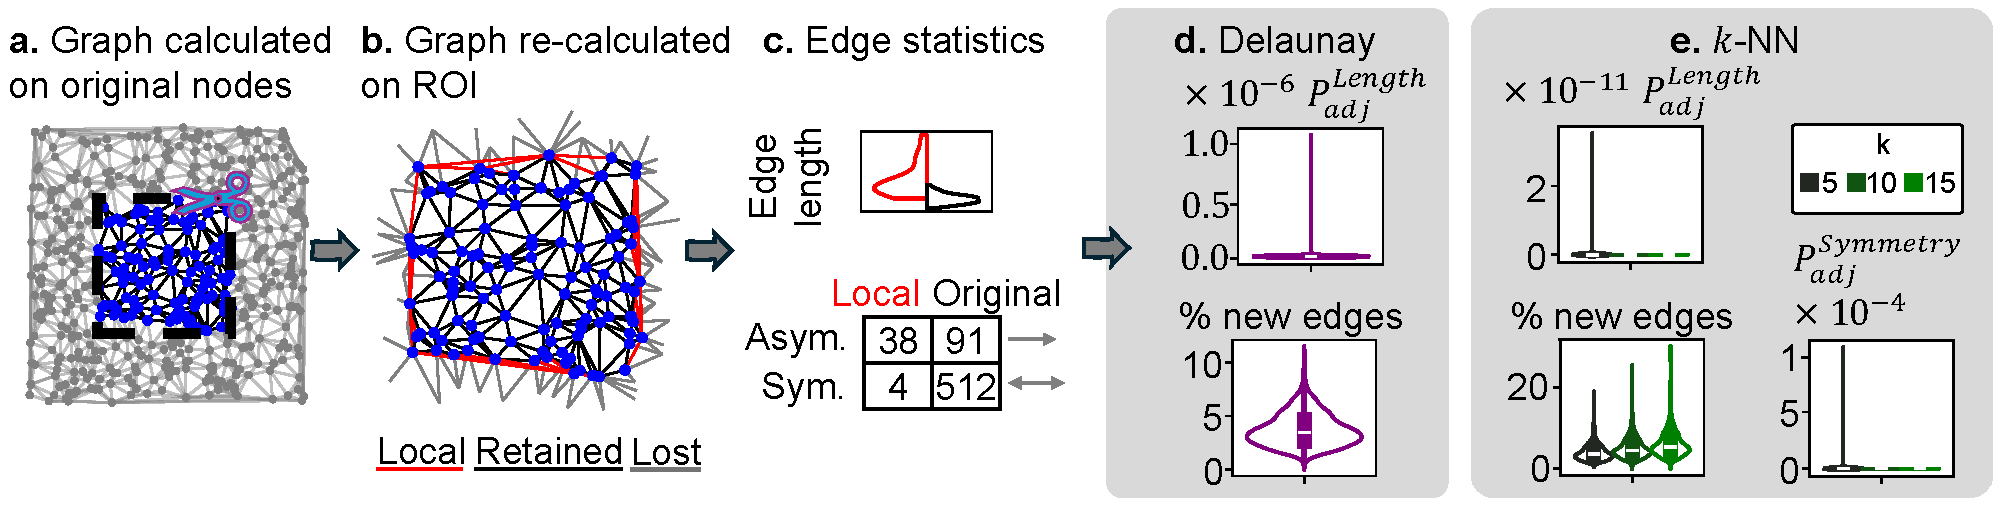
\includegraphics[width=0.9\linewidth]{figures/Fig1_del_knn.pdf}
    \caption{Truncation reshapes edge structure in proximity-induced graphs. \textbf{(a--c)} Procedure to characterize border effects on proximity-induced graphs computed on cell centroids from MIBITOF and Visium Spatial Transcriptomics data \citep{keren2018structured, mccaffrey2022immunoregulatory, piyadasa2026multi}. \textbf{(a)} The global graph $G_{global}$ is constructed on all centroids. \textbf{(b)} To simulate truncation, $G_{local}$ is recomputed on the subset of centroids within a ROI, partitioning edges into retained (black), lost (grey), and newly introduced local edges (red). \textbf{(c)} The length distributions of local and retained edges are compared using a Mann-Whitney U (MWU) test; for directed $k$-NN graphs, edge symmetry is additionally compared using Fisher's exact test. \textbf{(d,e)} Violin plots of the fraction of local edges and MWU $P$-values for Delaunay \textbf{(d)} and $k$-NN \textbf{(e)} graphs; panel (e) additionally shows Fisher's exact $P$-values for edge symmetry.}
    \label{fig:trunc}
\end{figure}

A proximity-induced graph operator $\mathcal{G}$ is in general not restriction-stable: for a finite point set $V \subset \mathbb{R}^2$ and its truncation $V' = \{ v \in V \mid v \in \text{ROI} \}$,
\[
    \mathcal{G}(V') \neq \mathcal{G}(V)\vert_{V'}.
\]
Recomputing the graph on a truncated vertex set therefore removes edges that existed globally and may introduce edges that would not exist in the full spatial domain. To characterize this effect empirically, we constructed proximity-induced graphs on centroids of segmented cells from MIBITOF data and on spot coordinates from Visium Spatial Transcriptomics data (see Methods). We defined the global graph $G_{global} = \mathcal{G}(V)$ (\Cref{fig:trunc}a) and the local graph $G_{local} = \mathcal{G}(V')$ (\Cref{fig:trunc}b) , and partitioned edges into three disjoint classes: edges retained after truncation ($E_{retained} = E_{global} \cap E_{ROI}$), edges present globally but lost in the ROI ($E_{lost} = E_{global} \setminus E_{ROI}$), and new edges formed by local recomputation ($E_{local} = E_{ROI} \setminus E_{global}$). We then compared the length and, for directed $k$-NN graphs, the symmetry of $E_{local}$ against $E_{retained}$ (\Cref{fig:trunc}c).

The results differed systematically across graph types (\Cref{fig:trunc}d,e). For Delaunay triangulations, $E_{local}$ comprised up to 10\% of all edges in $G_{local}$ (median 3.47\%) and were significantly longer than $E_{retained}$ across all samples. For $k$-NN graphs, the fraction of local edges increased with $k$ (medians: $k=5$: 3.55\%; $k=10$: 4.48\%; $k=15$: 5.32\%), reaching up to 24\% of edges for $k=15$. In all samples, $E_{local}$ were significantly longer and significantly more asymmetric than $E_{retained}$, with the asymmetry reflecting the directional nature of $k$-NN graphs at boundaries. For radius graphs, $E_{local} = \emptyset$: no new edges were introduced, and all topological changes were captured by $E_{lost}$, consisting of edges that crossed the ROI boundary. Together, these results demonstrate that recomputing proximity graphs on truncated domains constitutes an inherent geometric artifact, introducing disproportionately long and, in $k$-NN graphs, asymmetric edges at the boundary.

\subsection*{Centrality measures are disturbed at borders in proximity-induced graphs}
\begin{figure}[ht]
    \centering
    \includegraphics[width=\linewidth]{figures/Fig2_rel_ll_effect.pdf}
    \caption{Border distance systematically predicts node centrality. \textbf{(a--d)} Concept illustrated on a representative image. \textbf{(a)} Cell centroids colored by closeness centrality, showing lower values near the border. \textbf{(b)} Same centroids colored by Euclidean distance to the convex hull. \textbf{(c)} Closeness centrality plotted against border distance for all nodes, with the four candidate fits overlaid (constant, piecewise linear, exponential saturation, Michaelis-Menten). \textbf{(d)} The AIC-best model is selected; effect strength and half-life are extracted from its parameters to characterize the magnitude and spatial reach of the border effect. \textbf{(e,f)} Results across all datasets and graph types ($k$-NN with $k\in\{5,10,15\}$, radius graphs with $r\in\{0.03,0.04,0.05\}$, Delaunay). \textbf{(e)} Relative likelihood $\ell$ of the AIC-selected best fit over the constant baseline (y-axis) vs.\ AIC-weight entropy $H_{AIC}$ of the candidate models (x-axis); color indicates the selected model. High $\ell$ indicates a strong distance-dependent effect; high $H_{AIC}$ indicates no clear preference between saturation model flavors. \textbf{(f)} Effect strength vs.\ half-life, quantifying how severe the border effect is and how far it propagates into the tissue.}
    \label{fig:rel_ll}
\end{figure}

Having established that truncation alters graph topology at boundaries, we next asked whether this structural distortion propagates to node-level centrality measures. We computed Delaunay, $k$-NN ($k \in \{5, 10, 15\}$), and radius ($r \in \{0.03, 0.04, 0.05\}$, with coordinates normalized to $[0,1]$) graphs directly on the cell centroids from the same biological datasets, without additional truncation, as these centroids already reside in an extrinsically bounded space defined by the imaging field of view. One graph from an image containing only three cells was excluded. For each node $n$, we computed its Euclidean distance $d_n$ to the nearest point on the convex hull of all centroids as a proxy for distance to the border. We then calculated five centrality measures for each graph: degree, closeness, betweenness, clustering coefficient, and PageRank centrality.

To quantify the dependence of each centrality measure on border distance, we use \texttt{bosperrus} to fit four parametric models to the observed pairs $(d_n, C_n)$ for $n = 1, \dots, N$: a constant baseline (no border effect), a piecewise linear model (local effect up to a knot, then plateau), an exponential saturation model, and a Michaelis-Menten style model (see Methods). The saturation models are motivated by the expectation that border effects are strongest at the periphery and decay with increasing distance from the border, eventually reaching a stable interior value. For each graph and each centrality measure, \texttt{bosperrus} selects the best-fitting model by the Akaike Information Criterion (AIC) and computes two summary statistics: the relative likelihood $\ell$ of the best candidate model over the constant baseline, which quantifies how much evidence there is for a distance-dependent border effect, and the entropy $H_{AIC}$ of the AIC weights across candidate models, which quantifies whether one saturation model is clearly preferred over the others.

\Cref{fig:rel_ll}e,f shows the results across all datasets, graph types, and centrality measures. A distance-dependent border effect was the rule rather than the exception: the constant baseline was the AIC-best model only for degree and PageRank centrality in Delaunay graphs, and even there only in a minority of samples. For all other measure-graph combinations, a saturation model provided a substantially better fit, with relative likelihoods $\ell$ well above one. The specific flavor of saturation model had little impact on model selection: $H_{AIC}$ was close to its maximum of one in the majority of cases, indicating that the saturation models were interchangeable in terms of AIC. Degree centrality in Delaunay and $k$-NN graphs showed a characteristically local effect pattern, with a steep rise close to the border followed by rapid saturation, consistent with the geometric observation that $E_{local}$ in these graph types is concentrated in a narrow border buffer. Closeness and betweenness centrality exhibited broader effects propagating further into the tissue interior, as reflected by larger half-life values (\Cref{fig:rel_ll}f), consistent with the global nature of path-based centrality measures.
\FloatBarrier

\subsection*{Fit-based correction improves correlation with ground truth}
\begin{figure}[ht]
    \centering
    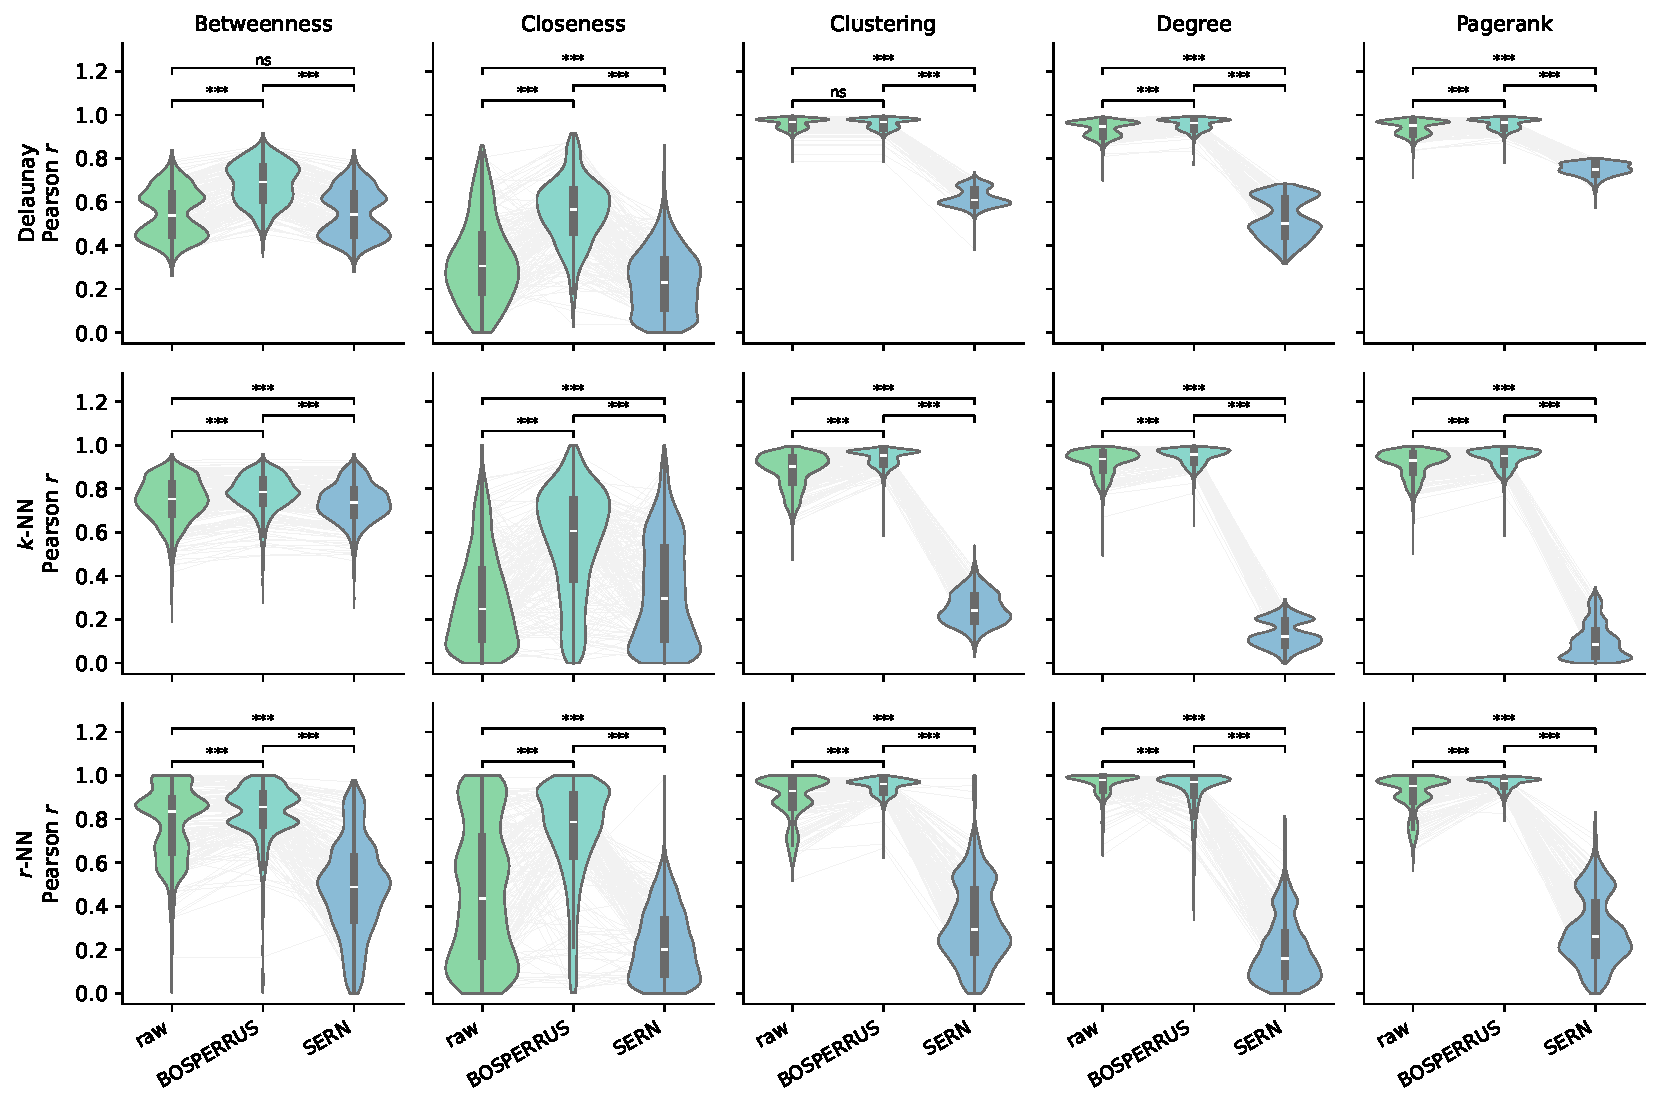
\includegraphics[width=\linewidth]{figures/Fig3_correlations_on_sphere.pdf}
    \caption{\textcolor{red}{Preliminary figure.} For each centrality measure (columns) and graph type (rows within each panel), bars show the fraction of simulation runs in which each method --- uncorrected $C_{ROI}$, \texttt{bosperrus}-corrected $\hat{C}_{ROI}$, or SERN-corrected $\hat{C}_{SERN}$ --- achieved the highest Pearson correlation with the ground-truth global centrality $C_{global}$. Results are aggregated over $12{,}600$ runs per centrality measure, spanning three node distributions, four cap sizes $g\in[1,2]$, three graph types, and all parameter combinations $k\in\{5,10,15\}$ and $r\in\{0.05,0.1,0.15\}$.}
    \label{fig:sphere_correlations}
\end{figure}

To evaluate whether the \texttt{bosperrus} correction recovers ground-truth centralities, we adopted a simulation strategy inspired by \citet{rheinwalt2012boundary}, using the unit sphere as a borderless reference geometry. We simulated $n=5{,}000$ nodes per run under three spatial distributions: uniform on the sphere, a single von Mises-Fisher (vMF) distribution ($\kappa=1$, random $\mu$), and a mixture of three vMF components ($\kappa\in\{1,3,5\}$, random $\mu$), designed to produce varying degrees of spatial clustering. From each configuration, we randomly cropped a spherical cap of geodesic radius $g\in[1,2]$ and treated the retained nodes as the ROI. Ground-truth centralities $C_{global}$ were computed on graphs built over all nodes; ROI centralities $C_{ROI}$ were computed on graphs restricted to the cap.

We evaluated all three graph types considered throughout this study — Delaunay triangulation, $k$-NN graphs ($k\in\{5,10,15\}$), and radius graphs ($r\in\{0.05,0.1,0.15\}$) — both globally and on the cap. \texttt{bosperrus} was applied to correct $C_{ROI}$ using the AIC-selected best fit, yielding corrected centralities $\hat{C}_{ROI} = C_{ROI} + \Delta(d)$, where the additive compensation term $\Delta(d) = C_{\text{plateau}} - C_{\text{model}}(d)$ shifts each node's centrality to the plateau of the fitted model (\Cref{eq:correction}). As a competitor, we computed $n=100$ spatially embedded random networks (SERNs) \citep{barnett2007spatially} as proposed by \citet{rheinwalt2012boundary}, retrieved their median centralities $C_{SERN}$, and obtained SERN-corrected values as $\hat{C}_{SERN} = C_{ROI} - C_{SERN}$. We assessed performance as the Pearson correlation of each corrected or uncorrected score with $C_{global}$, and for each run determined which method achieved the highest correlation. The full benchmark comprised $12{,}600$ runs per centrality measure, spanning all combinations of node distribution, cap size, graph type, and graph parameters.

\texttt{bosperrus} outperformed both the uncorrected scores and the SERN-based correction across the large majority of settings (\Cref{fig:sphere_correlations}). For Delaunay and $k$-NN graphs, \texttt{bosperrus}-corrected centralities achieved the highest correlation with $C_{global}$ in the majority of runs across all centrality measures. For radius graphs and degree centrality, uncorrected values marginally outperformed both correction methods in slightly more than half of runs, consistent with the observation that radius graphs do not introduce new local edges and therefore exhibit weaker and less systematic border artifacts. The SERN approach was consistently dominated by \texttt{bosperrus}, and showed signs of over-correction in several settings. Furthermore, computing 100 SERNs per sample represents a substantial computational overhead, as only the median is used for correction, leaving the variance of the ensemble unexploited.


%\subsection*{Modeling centralities in dependence of natural and artificial border separates truncation artifacts from structural differences}
%\paragraph{Hypothesis}
%\paragraph{Data}
%\cite{keren2018structured} maybe suitable, tumor and immune regions are defined via cells
%\cite{jackson2020single}
%\paragraph{Strategy}
%\paragraph{Results}

%\subsection*{Transfer of concept to physical geography}
%\paragraph{Hypothesis}
%Multi-border effects can be measured in physically-realized spatial graphs that are extracted from maps. 
%\begin{itemize}
%    \item Example: \url{https://beta-naptan.dft.gov.uk/} dataset. 
%    \item Nodes: UK train stations, bus stops, etc.
%    \item Edges: UK train lines, bus lines, etc. 
%    \item "Natural" borders: Ocean
%    \item "Artificial" borders: Country borders (England/Scotland/Wales) or county borders. 
%    \item Question: does county-level (or country-level) organization of public transport break networks at %county borders? 
%\end{itemize}
%\paragraph{Data}
%\url{https://beta-naptan.dft.gov.uk/} dataset. 
%Data for borders?
%\paragraph{Strategy}
%Model centralities as $C(d_{ocean}, d_{county-border})$. Identify and correct effect of natural border to %isolate effect of artificial border. 
%\paragraph{Results}

\subsection*{Applications in biological domain}
\begin{itemize}
    \item Proximity-induced graphs:
    \begin{itemize}
        \item Border effects in Visium HD expression?
        \item Border effects in neighborhood-enrichment?
    \end{itemize}
    \item Physically realized graphs:
    \begin{itemize}
    \item Effect on centralities intrinsic border (HRF?)
    \item Effect on centralities extrinsic border
    \end{itemize}
\end{itemize}
\subsection{Applications in other domains}
\begin{itemize}
    \item Brightkite data: influence of "urbanity" on centrality scores, influence of time zone on centrality scores
    \item Geodata: maybe from \cite{gil2015examining}, or UK public transport -> political versus natural borders
    \item Weather data: from \cite{rheinwalt2012boundary}??
\end{itemize}
\FloatBarrier

\section*{Methods}
\subsection*{Proximity-induced graphs}
We consider three proximity graph operators:

\begin{itemize}
    \item \textbf{Delaunay graph:}
    \[
    (u,v) \in E 
    \quad \Longleftrightarrow \quad
    \exists \text{ a circle passing through } u,v 
    \text{ whose interior contains no point of } V.
    \]

    \item \textbf{$k$-nearest neighbor ($k$-NN) graph (directed):}
    For fixed $k \in \mathbb{N}$,
    \[
    (u,v) \in E 
    \quad \Longleftrightarrow \quad
    v \text{ is among the } k \text{ closest points to } u 
    \text{ in Euclidean distance}.
    \]

    \item \textbf{Radius graph:}
    For fixed radius $r>0$,
    \[
    (u,v) \in E 
    \quad \Longleftrightarrow \quad
    \|u - v\| \le r.
    \]
\end{itemize}

\subsection*{Models}
\begin{itemize}
    \item a constant fit (one parameter)
    $$C_{const}(d) = a = \text{const.},$$
    \item a piece-wise linear fit with one elbow (three parameters)
    $$C_{pie-lin}(d) = \begin{cases}
    m d + c, & d \le b \\
    m b + c = \text{const.}, & d > b
    \end{cases},$$
    \item an exponential saturation model (three parameters)
    $$C_{exp}(d) = a (1-e^{-bd}) + c$$
    \item a Michaelis-Menten style model:
    $$C_{MM}(d) = \frac{a*d}{b+d} + c$$
\end{itemize} 

\subsection*{Quality of fits}
\begin{itemize}
    \item the \textbf{maximized log-likelihood} $\ell$ of each fitted model:
    \begin{itemize}
        \item Assuming independent, normally distributed residuals with constant variance, 
        $$ \varepsilon_n = C_n - \widehat{C}_n \sim \mathcal{N}(0,\sigma^2), $$
        \item we estimate the variance via the mean squared error,
        $$ \widehat{\sigma}^2 = \frac{1}{N} \sum_{n=1}^{N} (C_n - \widehat{C}_n)^2.$$
        \item The maximized log-likelihood of the model is then
        $$\ell = -\frac{N}{2} \left( \log(2\pi \widehat{\sigma}^2) + 1 \right).$$
    \end{itemize}
    \item the Akaike Information Criterion (AIC) $$\mathrm{AIC} = 2(k+1) - 2\ell,$$ to compare models while penalizing model complexity ($k$ shape parameters; the additional $+1$ accounts for the residual variance $\widehat{\sigma}^2$ treated as an estimated parameter)
    \item the relative likelihood of each candidate model against the constant baseline model, divided by the number of nodes, 
    $$ R_{scaled} = \exp(\frac{\mathrm{AIC}_{\mathrm{const}} - \mathrm{AIC}_{\mathrm{model}}}{2N}),$$
    where $N$ denotes the number of nodes in the graph. This normalization accounts for the fact that AIC scales linearly with sample size, enabling comparisons across graphs of different sizes,
    \item the Akaike weights of the two candidate models (exponential, and piece-wise linear), 
    $$w_i= \frac{R_{i}}{\sum_{j=1}^{2}R_{j}},$$
    interpreted as the relative support for model $i$,
    \item the normalized Shannon entropy of these Akaike weights, 
    $$H_{\mathrm{AIC}} = - \frac{1}{\log 2} \sum_{i=1}^{2} w_i \log w_i,$$ 
    which quantifies the uncertainty of model selection. Values close to $0$ indicate strong evidence for a single model, whereas values close to $1$ indicate comparable support for multiple models.
\end{itemize}

\begin{itemize}
    \item the fraction of affected nodes:
    $$f= \frac{1}{N}\sum_{i=1}^{N}d_i<d_\alpha,~\text{with}~
    d_\alpha:\alpha-\text{convergence}
    $$ 
    \item the observed half-life:
    $$d_{50}={C}^{-1}\left(\ \frac{C\left(\operatorname{d}_{min}\right)+C\left(\operatorname{d}_{max}\right)\mathrm{\ } }{2}\ \right)$$
    \item the observed effect strength:
    $$e= \frac{C\left(d_{min}\right)-C\left(d_{max}\right)\mathrm{\ } }{C\left(d_{min}\right)+C\left(d_{max}\right)+\epsilon}$$
\end{itemize}


\subsection*{Data availability}
\begin{itemize}
    \item Data used for effects of truncation on proximity-induced graphs:
    \begin{itemize}
        \item \cite{keren2018structured}
        \item \cite{mccaffrey2022immunoregulatory}
        \item \cite{piyadasa2026multi}
        \item all datasets in squidpy version 1.2.2's squidpy.datasets.visium

    \end{itemize}
\end{itemize}

\section*{Acknowledgments}

\bibliography{sample}

\end{document}